\begin{spacing}{1.5}
\phantom
\phantom
\phantom
\phantom
\section{Literature Review}
\phantom
\phantom
The debate over Ontario's forest fire suppression policy has centered on the credibility of a retrospective study carried out by fire managers at Ontario's Ministry of Natural Resources (Ward and Tithecott 1993). This study has been cited many times in support of the supposed 'effectiveness' of fire suppression, despite being an internal OMNR document, not peer-reviewed science (see Li \emph{et al}. 1996; Welsh and Venier 1996; OMNR 1997; Bourgeau-Chavez \emph{et al}. 2000). The study has faced criticism, most notably from fire ecologists (Johnson \emph{et al}. 2001; Miyanishi and Johnson 2001; Miyanishi \emph{et al}. 2002). While, Ward and Tithecott have sought to defended their original analysis (Ward, Tithecott and Wotton 2001), the case for effective fire suppression in Ontario remains in dispute.

\subsection{Ward and Tithecott's Original Thesis}
Ward and Tithecott's original report discussed the role played by fire suppression in managing Ontario's forests (Ward, Tithecott and Wotton 2001:1468). Part of their analysis dealt specifically with the impact of fire-suppression activities in regulating fire--size distributions. \\

\noindent The authors began with a simple hypothesis:

\begin{quote}
``{\it A fire suppressed when small, would have otherwise grown to become large in the absence of that suppressive action}'' (Ward, Tithecott and Wotton 2001:1469).
\end{quote}

\noindent From this hypothesis they made a prediction--given two similar forests, one with fire suppression and one without, the forest with suppression would have more small fires, and fewer large fires than in the unsuppressed forest (Ward, Tithecott and Wotton 2001:1469).

\clearpage

\noindent To assess the validity of this prediction, Ward and Tithecott (1993) compared the fire distributions between a forested area with some degree of protection, and an area without, over the same 15 year period. The fire--size distribution in areas with fire protection was calculated for Ontario's 'Intensive' and 'Measured' fire management zones (i.e., those areas with fire suppression), using annual fire statistics over the period 1976 to 1990, derived from provincial fire management records in the Ontario Ministry of Natural Resources (OMNR) fire database (Ward, Tithecott and Wotton 2001:1473). Data drawn from the 'Extensive' fire management zone, in which fires are generally (though not exclusively) not suppressed, was used for what Ward and Tithecott (1993) argue is a ``\emph{surrogate indicator of the natural distribution of fires by size class in the pre-suppression era}.'' \\

\noindent The results were presented as plots of the mean annual numbers of fires by size--class, in the unprotected zone (i.e., Ontario's Extensive fire management zone) and the protected zones (i.e., Ontario's Intensive and Measured fire management zones) (see \emph{Figure~\ref{fig3}}), (Ward and Tithecott 1993, cited in Miyanishi and Johnson 2001:1463). These graphs show a relatively flat distribution for the area without fire suppression (\emph{Figure~\ref{fig3}a}), and a highly right--skewed distribution for those areas with fire suppression (\emph{Figure~\ref{fig3}b}), (Bridge, Miyanishi and Johnson 2005:43). \\

\begin{figure}[h!]
  \centering
    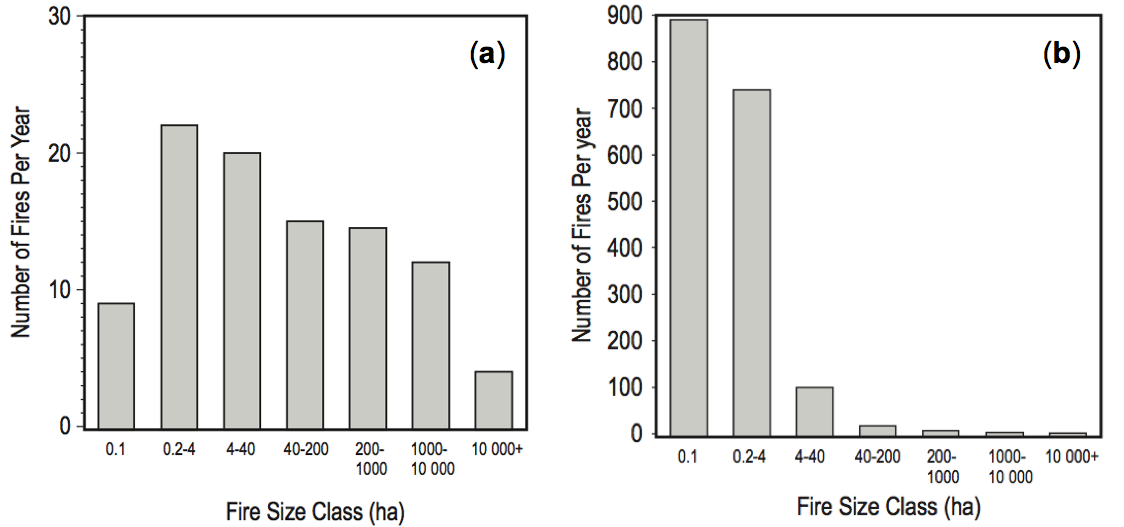
\includegraphics[width=1\textwidth]{media/fig3}
      \caption[Distribution of mean annual fire--size classes]{\emph{Distribution of the mean annual fire--size classes (\emph{ha}) in (\textbf{a}) Ontario's unprotected Extensive Fire management zone, and (\textbf{b}) protected Intensive and Measured Fire management zones (1976--1990), (adapted from Ward and Tithecott 1993, cited in Miyanishi and Johnson 2001:1463).}}
        \label{fig3}
\end{figure}

\clearpage

\noindent Ward and Tithecott (1993) interpreted these results as follows: \emph{Figure 1a} shows a natural fire regime, similar to the pre--suppression era, in which fires would have been naturally distributed across a wide range of size classes (Ward, Tithecott and Wotton 2001:1473). Whereas \emph{Figure 1b} shows very few fires reaching the larger class--sizes. The explanation given for this difference in the shape of the distribution of fire sizes is that, unlike in the unprotected zone, fire suppression in the Intensive and Measured fire management zones prevents many smaller fires from becoming large, compared with what would have been observed without fire suppression (Ward, Tithecott and Wotton 2001:1473). Thereby, fire suppression has skewed the number of fires recorded towards the smaller fire size classes, into a 'J' shaped distribution (Bridge, Miyanishi and Johnson 2005:43). \\

\noindent The same dataset was also presented in Ward and Mawdsley (2000). However, here the protected and unprotected fire management zones were combined into a single graph showing the annual number of fires as a  percentage (\emph{Figure~\ref{fig4}}). The same conclusion was drawn however, in that fire suppression in the protected zone is creating far fewer moderate-- and large--sized fires than in the unprotected zone (Ward and Mawdsley 2000). \\

\begin{figure}[h!]
  \centering
    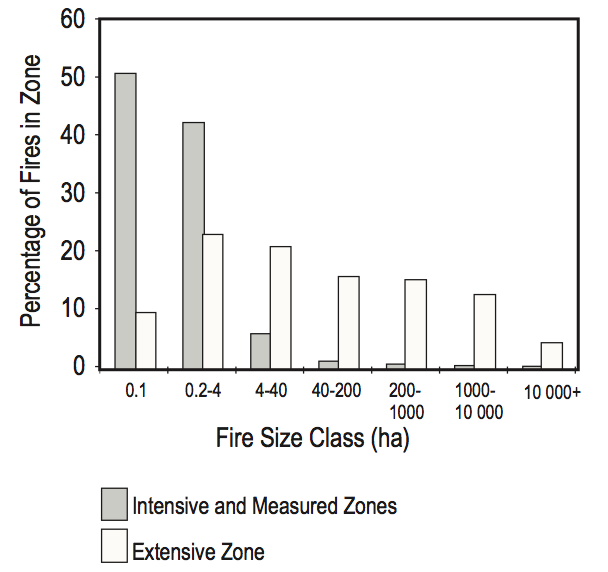
\includegraphics[width=0.7\textwidth]{media/fig4}
      \caption[Distribution of percentage of fires by size-class]{\emph{Distribution of percentage of fires by size class in Ontario (1976--1990) for the unprotected and protected fire management zones (adapted from Ward and Mawdsley 2000:73).}}
        \label{fig4}
\end{figure}

\clearpage

\noindent Ward and Tithecott argue that these results show fire suppression has indeed ``\emph{reduced the overall area burned in the protected forest, compared with what would have occurred in the absence of fire suppression}'' (Ward, Tithecott and Wotton 2001:1479), and therefore, prove the effectiveness of fire suppression in Ontario (Ward and Tithecott 1993; Ward, Tithecott and Wotton 2001; and Ward and Mawdsley 2000).

\subsection{Fire--Ecologist's Critiques}

Fire--ecologists have argued however, that Ward and Tithecott's analysis contains several fatal flaws (Miyanishi and Johnson 2001; Johnson \emph{et al}. 2001; and Miyaishi \emph{et al}. 2002). 

\subsubsection{Difference in Fire Detection Resolution}

In the first case, Miyanishi and Johnson (2001:1463) are suspicious of the data presented in \emph{Figure~\ref{fig3}}, on page~\pageref{fig3} (Ward and Tithecott 1993, cited in Miyanishi and Johnson 2001:1463), which suggests a great disparity in the annual number of fires between the protected Intensive and Measured zones ($\sim$2000 fires per year), and the unprotected Extensive zone (only $\sim$100 fires per year). Furthermore, the number of small fires (<4\emph{ha}) in the Extensive zone (\emph{Figure~\ref{fig3}a}) seems extremely small (at only $\sim$30 fires per year), especially considering the vast size of the area in question. \\ 

\noindent Ward and Tithecott (1993) noted that they may have underestimated the number of small fires in the Extensive zone, as the detection of fires in this zone is thought to be biased towards larger fires. This is common error in estimating fire occurrences (Ricotta \emph{et al}. 1999; Holmes \emph{et al}. 2004; Telesca \emph{et al}. 2005), especially in areas where small fires are not considered important enough to record (Ward \emph{et al}. 2001; Bridge \emph{et al}. 2005). It is therefore possible that these discrepancies are due to the fact that in the sparsely populated Extensive zone, many small fires are simply never detected. Miyanishi and Johnson (2001:1464) conclude that ``\emph{any comparison of the numbers of small fires between the two zones cannot be valid due to these differences in detection resolution}.'' \\

\noindent However, Ward and Tithecott believe that their original analysis is still valid, as the area burned by small undetected fires is relatively insignificant compared to the overall area burned each year, and therefore, recording their full impact is not strictly required to understand the role of fire suppression in Ontario (Ward and Tithecott and Wotton 2001:1473).

\subsubsection{Misrepresenting the Distribution of Larger Fires}

Miyanishi and Johnson's (2001:1464) second critique relates to the way in which the comparison between the number of fires in the protected and unprotected zones has been presented. They note that the x--axis on the two graphs in \emph{Figure~\ref{fig3}}, on page~\pageref{fig7} (i.e., The number of fires per year) are plotted over two different scales (0--30 in \emph{Figure~\ref{fig3}a}, and 0--900 in \emph{Figure~\ref{fig3}b}). This  gives the impression that there are fewer large fires in the protected zone than in the unprotected zone. However, when the Ontario dataset is plotted with the x--axis on the same scale, as Miyanishi and Johnson (2001:1464) have shown below (\emph{Figure~\ref{fig5}}), there is little difference between the two zones in the number of moderate-- and large--sized fires (i.e., fires >40 \emph{ha}). \\

\begin{figure}[h!]
  \centering
    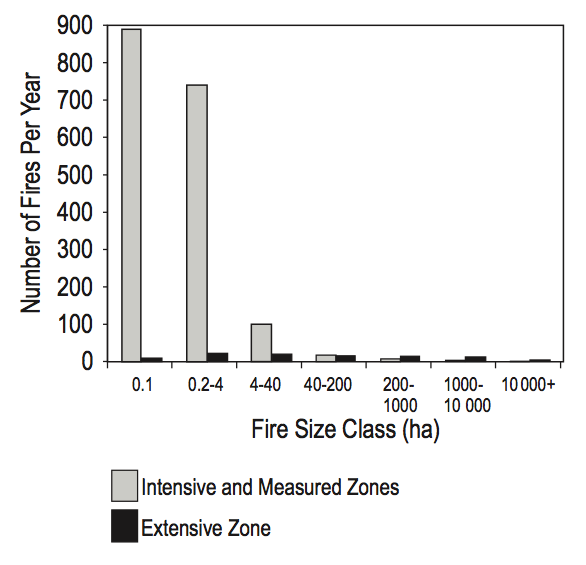
\includegraphics[width=0.7\textwidth]{media/fig5}
      \caption[Distribution of mean annual fire sizes, using same vertical axis]{\emph{Distribution of mean annual fire sizes (\emph{ha}) within Ontario's unprotected Extensive Fire management zone and protected Intensive and Measured Fire management zones (1976--1990) using the same scale for the vertical axis. Redrawn from data presented in Ward and Tithecott (1993), (adapted from Miyanishi and Johnson 2001:1464).}}
        \label{fig5}
\end{figure}

\clearpage

\noindent While this mistake was corrected in Ward and Mawdsley (2000:73), the x--axis was plotted as a percentage of the number of fires in each zone (see \emph{Figure~\ref{fig4}}, on page~\pageref{fig4}). Miyanishi and Johnson (2001:1464) argue that this representation of the data can also give a mistaken impression that there are fewer large fires in the protected zones than in the unprotected zone. As previously noted, the data on the number of small fires occurring in the unprotected zone is likely to be censored, therefore, those missing small fires would in effect, skew the distribution towards larger fire classes. Miyanishi and Johnson (2001:1464) conclude, contrary to Ward and Tithecott (1993), that the Ontario dataset shows fire suppression to have not significantly changed the observed distribution of medium-- and large--forest fires.

\subsubsection{Lack of Consideration of Environmental Variables}

As noted in Miyanishi \emph{et al.} (2002), the analysis presented in Ward and Tithecott (1993) and Ward et al. (2001) does not adequately consider the  differences that exist between the various fire management zones. It is implicitly assumed in the research design of these studies, that the fire management zones differ only in their fire--suppression policies, and therefore, inferred that the differing levels of fire suppression must account for the differences seen in the distribution of large forest fires (i.e., that the distribution of forest fires is dependent on the fire suppression strategy being employed). The problem, however, is that Ontario's fire--protection zones conform to a general north--south gradation in several environmental variables associated with forest fire dynamics, such as climate, topography, tree species, ignition sources and human activity (Miyanishi \emph{et al}. 2002:1177), as well as longitudinal gradients in humidity and fire frequency (Beverly and Martell 2005; Hills 1959; Suffling 1995). As such, the spatial variation of these variables could also have a causal link to the distribution of fires and, under ideal scientific conditions, should have been controlled for in the original research design. Unfortunately, in this case quantitative disturbance records from Ontario's pre--suppression era do not exist (Ward, Tithecott and Wotton 2001:1470), making a comparison of fire size distributions in a single fire management zone, before and after a substantial period of fire suppression unworkable.

\clearpage

\subsubsection{Stochastic Nature of Forest Fires}

The final problem outlined in Miyanishi \emph{et al}. (2002), relates to a more fundamental issue with retrospective statistical research. They argue that the extreme size, and stochastic nature of forest fires in boreal forests (see Weir \emph{et al}. 2000), leads to a very high annual variation in area burned. The occurrence (or omission) of a single large fire can therefore, have a significant effect on the results of any statistical analysis (Miyanishi \emph{et al}. 2002:1178). This is especially true of studies from which the data covers only a relatively short time period. Miyanishi \emph{et al}. (2002:1178) cite an example by Bridge (2001), in which the estimates of average annual burn rates were compared, based on 24 years (1972--1995) versus 75 years (1921--1995) of fire data in Ontario. Given that the analysis was using partially the same data, one would expect the estimates to be fairly similar. Bridge (2001) however, found these estimates could differ by several orders of magnitude. Miyanishi \emph{et al}. (2002:1178) also carried out their own analysis of average annual burn rates in Ontario, this time based on 13 years (1976--1988) versus 41 years (1955--1995) of fire data. They found that due to the very large fires in 1956 and 1961, which where not included in the shorter dataset, the estimated average annual burn rates differed wildly based on the omission of just these two years data.

\subsection{Defining of Fire Suppression Effectiveness}

While both Ward and Tithecott (1993) and Miyanishi \emph{et al}. (2001) agree that the objective of fire suppression is to reduce the area of a forest burned,  Cumming (2005:781) argues that neither have been able to developed a workable definition to measure this effect. \\

\noindent Fire ecologists are typically concerned with how the suppression of wildfires effects the structure of boreal forest. This is usually measured by the change in mean annual burn rate ($\sigma$), with fire suppression expected to reduce this statistic (Van Wagner 1978). While even small changes in $\sigma$ can have enormous ecological significance, this effect can only be estimated over very long periods of time, as some causal factors are related to changes in climate over the last 200 years (Bergeron \emph{et al}. 2004).

\clearpage

\noindent Unfortunately, while national fire statistics have been recorded since 1918 in Canada, large swathes of the remote northern regions of Ontario were not documented prior to the 1950s (Murphy \emph{et al}. 2000; Stocks \emph{et al}. 2002).  Therefore, one must conclude that the empirical data available in Ontario is simply inadequate for determining the effect of fire suppression using this method (Miyanishi \emph{et al}. 2002:1178). \\

\noindent Cumming (2005:773) argues that a definition of 'effectiveness' only needs to be relative to its objectives. In this case, the objective of fire managers in Ontario is to reduce the proportion of 'large' fires (i.e., those fires on which suppression has failed) in fire management zones with aggressive fire suppression policies (Martell 2001, cited in Cumming 2005:781). Therefore, one could argue that an effective fire suppression policy  requires that the observed proportion of large fires in areas with aggressive suppression only be lower than in those areas without. \\

\noindent Cumming (2005) has demonstrated this method by comparing the proportions of large fires between areas with contrasting fire management strategies in Alberta, while controlling for other factors (both spatial and temporal) likely to affect this distribution. He believes this effect is best measured as a distribution of the the odds that a randomly chosen fire will be suppressed (Cumming 2005:781).

\subsection{Considerations for Future Research}

While the case for effective fire suppression in Ontario has not been settled, several important observations can be made:

\begin{description}
\item[(i)]
Quantitative disturbance records from Ontario's pre--suppression era do not exist, making a direct comparison of a single area, with and without fire suppression unworkable. (see \emph{Chapter 2.1}).
\item[(ii)]
The difference in fire detection resolution between the unprotected and protected fire management zones also makes a comparison unworkable (see \emph{Chapter 2.2.1}).
\item[(iii)]
The results of any statistical analysis need to be presented in a way that does not distort the data (see \emph{Chapter 2.2.2}).
\item[(iv)]
Other differences between the fire management zones must be controlled for in any statistical analysis (see \emph{Chapter 2.2.3}).
\item[(v)]
Larger datasets will give more accurate results (see \emph{Chapter 2.2.4}).
\item[(vi)]
The definition of fire suppression effectiveness needs to be related to its objectives (see \emph{Chapter 2.3})
\end{description}

\noindent In considering further research on the impact of fire suppression, each of these points should be taken into account at the research design stage of the analysis.

\end{spacing}
\clearpage
